
%(BEGIN_QUESTION)
% Copyright 2015, Tony R. Kuphaldt, released under the Creative Commons Attribution License (v 1.0)
% This means you may do almost anything with this work of mine, so long as you give me proper credit

\noindent

\vskip 5pt


\textbf{Arbidsoppdrag -- introdusjon}

$$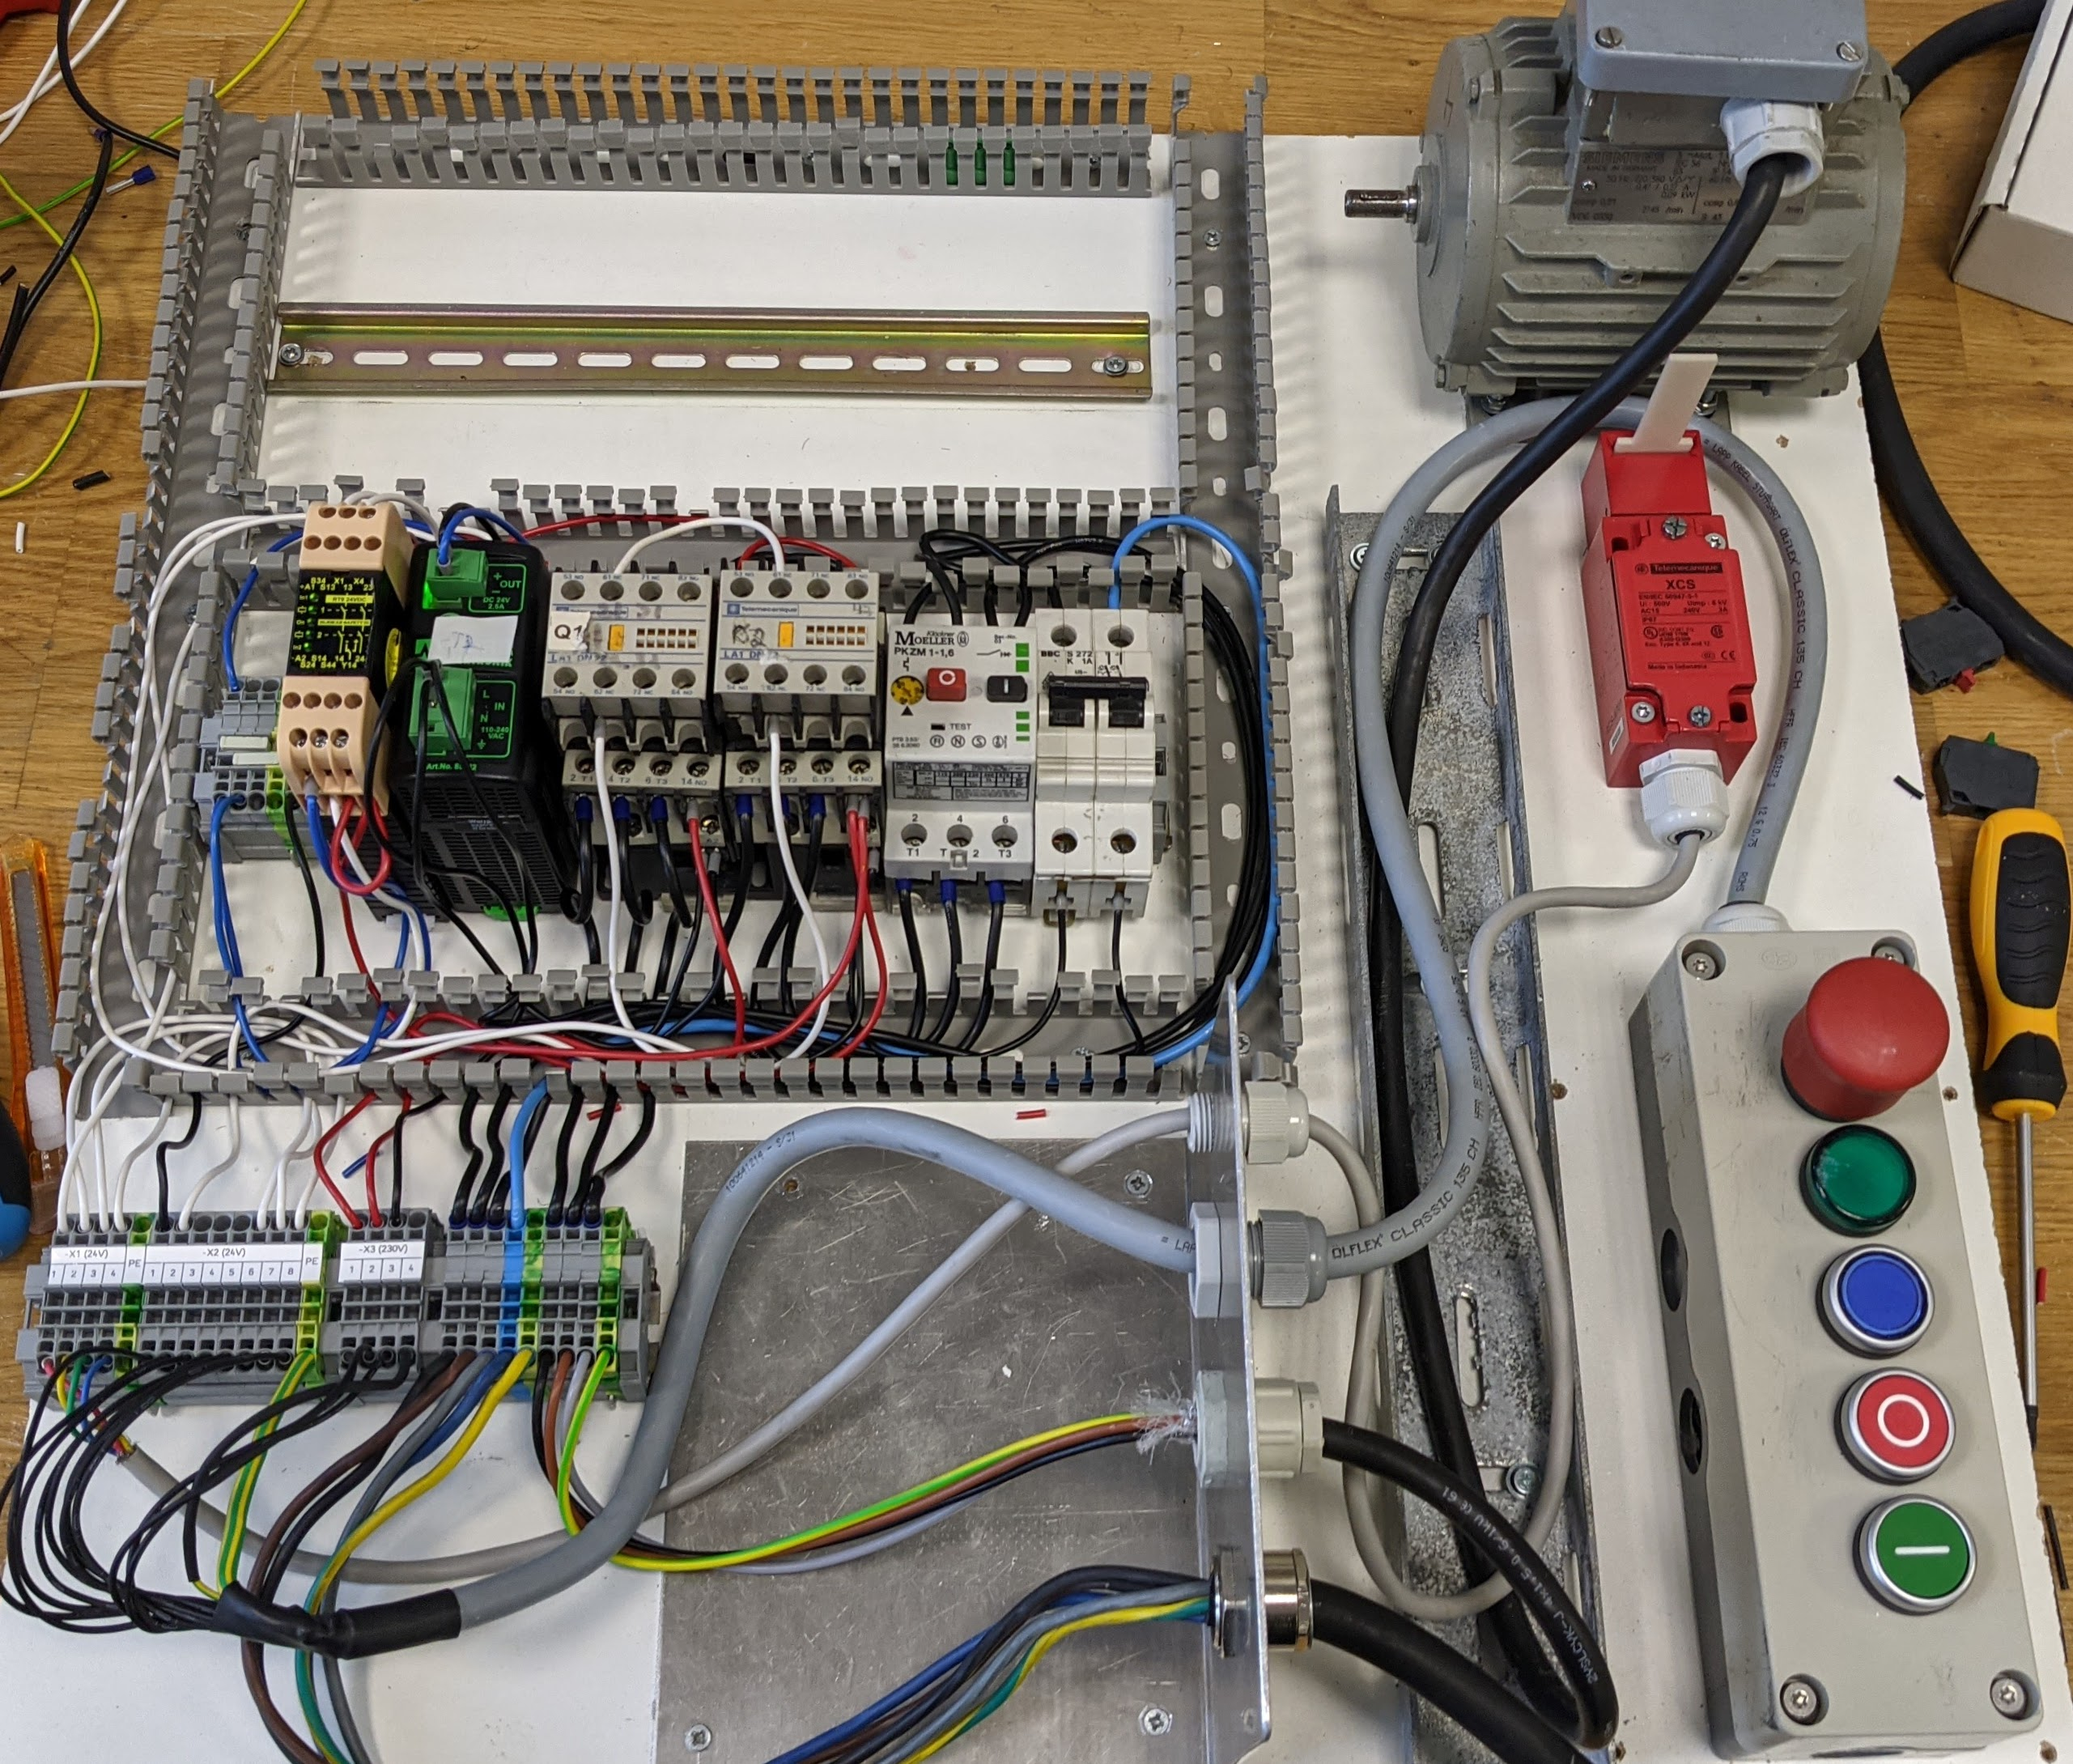
\includegraphics[width=13cm]{i04821x01.jpg}$$\\

Dette arbeidsoppdraget handler om sikkerhetsrelaterte deler av styre system. Du skal koble opp styrekrets til en tenkt maskin som er beskyttet med vern. Et bevegelig vern gir tilgang til maskinen. Det beveglige vernet overvåkes av en bryter som skal kobles til et Jokab RT9 sikkerhetsrele. \\ 

\begin {itemize}
\item Sikkerhetsrelatert stopp utløst av beveglig vern.
\item Manuel Reset
\end {itemize} 

Som et komplementært sikkerhetstiltak skal det monteres en nødsopp bryter. Det må også være vanlig drifts start og stopp. 

$$\includegraphics[width=13cm]{i04821x02.eps}$$\\

\vskip 10pt 
\textbf{Arbidsoppdrag -- teorioppgaver}

Oppgaver fra Kap 4
\begin{itemize}[noitemsep]


\item Er en sikkerhetsfunksjon i styresystemet første valget ved konstruksjon av maskiner?
%Nei første prioritet ved design av an maskin er å konstruere den slik at det ikke er behov for sikkerhetsfunksjoner. Om dette ikke er mulig bygges vern mot farene. Sikkerhetsfunksoner i styressystemet er ofte en del av dette vernet. F.eks. en bevegelig dør. 

\item Hva er en sikkerhetsfunksjon?
%En sikkerhetsfunksjon i styresystemet er en funksjon som skal bidra til å redusere risikoen ved en identifisert fare med maskinen

\item Hva står PL for?

%PL står for Preformance Level dette forteller noen om sansynligheten for at en sikkerhetsfunksjon virker når det er behov for en. 

\end{itemize}
	
	

\vskip 10pt 
Oppgaver fra Kap 5. 
\begin{itemize}[noitemsep]



	\item Gjelder EC machinery Directive i norge? Eventuelt hvilken lov er det implementert i?
%Den gjelder i norge som en del av EØS avtalen og er implementert i forskrit om maskiner. 


	\item Hvilken sikkerhetsstandard er viktig grunnlag for maskin direktivet?
%EN ISO 12100. Dette er en veldig generell standard som brukes for utgangpunkt for alle. Det finnes også B type standarder som omhandler spesiele deler av en maskin f.eks. EN 60204-1 som omhandler elektrisk utstyr i maskiner eller EN ISO 13849-1 som gjelder sikkerhetsrelaterte deler av styresystemer. Den siste standarden er C type standarder som gjelder for spesielle maskintyper f. eks. roboter. 

	\item Hva er en Type C standard under maskindirektivet?
%Det er en type standard som gjeler en maskin type. Når du skal konstruer en maskin må en alltid først sjekke om det finnes en C-type standard å følge. 

	\item Beskriv prosedyren for risikoreduksjon av en maskin. 
%		○ Bestemm grensene til maskinen
%		○ Identifiser farene
%		○ Estimer risikoen
%		○ Eveluer risikoen
%		○ Er risikoen lav nok? Ja/Nei (Ja slutt)
%		
		

	\item Hvordan finner en frem til nødvendig sikkerhetsfunksjoner
%For hver fare som er identifisert kommer en opp med en sikkerhetsfunksjon f.eksk. Vern og så vurderer en på nytt om risikoen er tilstrekkelig redusert. 

	\item Hvilke sikkerhetsfunksjoner er definert i EN ISO 13849-1
%		○ Sikkerhetsrelatert stoppfunksjon fra et bevegelig vern
%		○ Manuell resett
%		○ Start/restart
%		○ Manuell styring i faresone
%		○ Hold ut run
%		○ Enable (f.eks. knappen på sigen av robotkontrolleren)
%		○ Beskyttelse mot uventetoppstart ved operatør arbeid i faresone
%		○ Funsjon for å frigjøre personer som sitter fast. 
%		○ Isolasjon av frakobling av energi (elektrisk, mekanisk, hydraulisk, pneumatisk)
%		○ Styremodus. 
%		○ Utførelse av nødstopp. 

	\item Hvordan bestemmer PLr for en sikkerhetsfunksjon. 

\end{itemize}
\vskip 10pt 
\textbf{Arbidsoppdrag -- planlegging}\\
\\
Manualer 
\\
\url {https://cdn.logic-control.com/docs/abb-jokab-safety/06. Safety Relays.pdf}
\\
\url {https://www.dguv.de/medien/ifa/en/pub/rep/pdf/reports-2019/report0217e/rep0217e.pdf}
\\
\underbar{Tabell over fullførte oppgaver. }

% No blank lines allowed between lines of an \halign structure!
% I use comments (%) instead, so that TeX doesn't choke.
\begin{center}
\begin{tabular}{ | m{8cm} | m{1cm}| m{2cm} | } 
\hline
\multicolumn{3}{|c|}{Liste over utstyr som du tranger} \\
\hline
Utstyr	& Plass & sjekk \\ 
\hline
\hline
	Jokab RT9 & & \\ 
	\hline
	24V strømforsyning &&\\
	
	\hline
\end{tabular}
\end{center}
\vskip 10pt 
\textbf{Arbidsoppdrag -- gjennomføring}

\begin{center}
\begin{tabular}{ | m{8cm} | m{1cm}| m{2cm} | } 
\hline
\multicolumn{3}{|c|}{Sjekkliste for lærer før oppkobling starter} \\
\hline
Utstyr	& Plass & sjekk \\ 
\hline
	Teorisprørsmål besvart &&\\
\hline
	Fremdriftsplan &&\\
\hline
	
	Verktøys- og utstyrsliste &&\\
\hline
	Risikovurdering &&\\ 	
	\hline
	Koblingsskjema for oppkobling &&\\
	\hline
\end{tabular}
\end{center}
\vskip 10pt 

\textbf{Arbidsoppdrag -- dokumentasjon}


\textbf{Arbidsoppdrag -- gjennomføring}

\begin{center}
\begin{tabular}{ | m{8cm} | m{1cm}| m{2cm} | } 
\hline
\multicolumn{2}{|c|}{Sjekkliste for lærer etter at sluttkontroll er utført} \\
\hline
Test	& sjekk \\ 
\hline
\hline

	Anlegget starter og stopper ved normal stopp &\\
	
	\hline
	Motor stopper når dørbryter eller nødstopp aktiveres&\\
	\hline
	Manuell resett virker i henhold til 13849-1 &\\
	\hline
	Sjekk om kontaktorer har brent seg virker. &\\
	\hline
	Sluttkontroll er utført og dokumentert &\\
	\hline
	Elev har ført logg på Teams&\\
	\hline
	Elev har Tegnet koblingsskjema &\\
	\hline

\end{tabular}
\end{center}
\vskip 10pt 















\underbar{file i04821 mal}
\vfil \eject
%(END_QUESTION)





%(BEGIN_ANSWER)


%(END_ANSWER)





%(BEGIN_NOTES)


%INDEX% Arbeisdoppdrag, Styresystemer, Nivå 1, Stasjon16, sikkerhetsrele 

%(END_NOTES)


